\documentclass[main.tex]{subfiles}
\begin{document}
\section{Analysis and Discussion}

We evaluate the results against the five hypotheses proposed. Statistical significance is determined using the Student's t-test and the Mann-Whitney U test, with a standard significance threshold of p < 0.05, indicating statistically significant results.

\textbf{(H1):} \emph{Power draw and execution time are linearly correlated}
\\
\begin{figure*}[h]
    \centering
    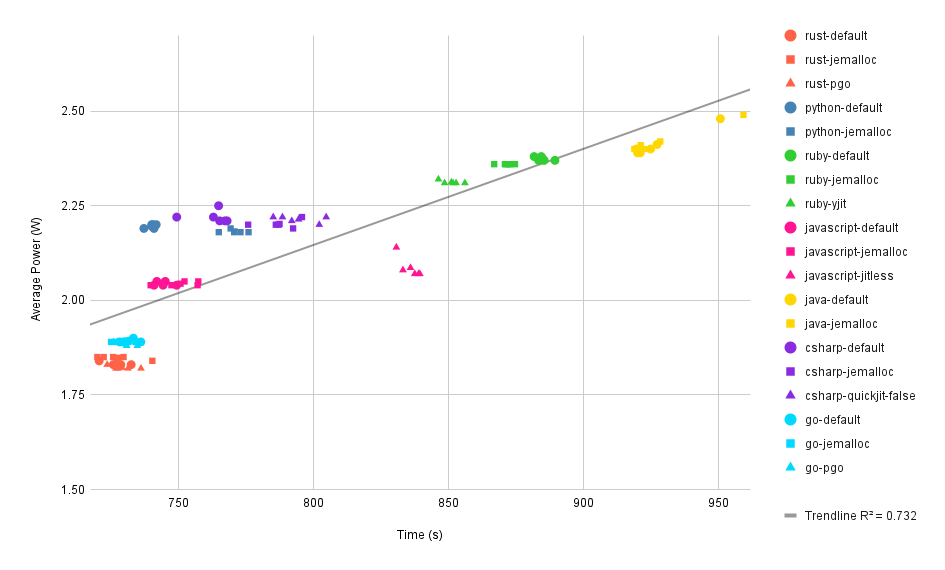
\includegraphics[width=\linewidth]{media/analysis/AveragePowerOverTime.png}
    \caption{Average Power for all experiments plotted over their Execution Time}
    \label{fig:analysis-energy-time-correlation}
\end{figure*}

In Figure \ref{fig:analysis-energy-time-correlation}, we see that there is a correlation between the execution time and the average power draw of each experiment. We also calculate a linear trendline with an R\textsuperscript{2} value of 0.732, which supports the correlation claim. To determine the strength and significance of the correlation, we use Pearson's Correlation between power draw and time for our results. For this, we see a correlation of 0.86 with a p-value of $3.09\times 10^{-29}$, indicating a very strong positive correlation  \cite{pearson-correlation-table}.

\textbf{(H2):} \emph{jemalloc lowers energy consumption compared to malloc}
\\
Our results from Table \ref{table:table-results} indicate that jemalloc generally leads to higher energy consumption compared to malloc, rejecting H2 in most cases.

\textbf{ruby-jemalloc:} Shows an energy reduction (-2.08\%, see $\Delta E$ in Table \ref{table:table-results}), supported by a p-value close to zero, meaning this reduction is statistically significant. Suggesting that using jemalloc with Ruby is beneficial for reducing the application's energy consumption. While jemalloc often increases energy consumption, in some implementations, like Ruby, it can have a beneficial effect.

\textbf{(H3):} \emph{JIT reduces energy consumption}
\\
The results strongly support our hypothesis that JIT reduces energy consumption. The ruby-yjit experiment, where we enabled JIT reduced the energy consumption, while the javascript-jitless and csharp-quickjit-false experiments where we disabled JIT, increased energy consumption. These results confirm that JIT plays an important role in optimizing energy consumption.

\textbf{(H4):} \emph{PGO reduces energy consumption}
\\
\textbf{rust-pgo \& go-pgo:} While we only have two PGO experiments, in both cases PGO resulted in lower energy consumption (-0.16\% for Rust and -0.72\% for Go, see $\Delta E$ in Table \ref{table:table-results}). That said, for our experiments, only the result for Go is statistically significant.

\textbf{(H5):} \emph{Some implementations will consume more energy than others, regardless of optimizations}
\\
The span of the implementations is large in terms of their energy consumption. Most implementations are distinct from one another, even when adjustments are made to the optimizations. The highest energy consumption for any Rust experiment iteration is less than 1,400 J, and the lowest for any Java iteration is above 2,200 J. This supports the hypothesis, since no matter which of the selected optimizations we use, Java will always consume more energy than Rust.

\textbf{javascript-jitless:} The only time a change in optimizations has a greater impact than the implementation itself is with javascript-jitless. The removal of JIT made the implementation slower, thus making it more comparable to some of the less performing implementations (see \ref{fig:boxplot}). From our results alone, it appears that implementation has a greater impact than the optimizations. 

\end{document}
